\section{OMNeT++}\label{sec:omnetpp}

\omnetpp{} is an extensible, modular, component-based C++ simulation library
and framework, primarily for building network simulators
\cite{omnetpp-simulation-manual}. \omnetpp{} is public-source and can be freely
used under the Academic Public License for non-profit purposes. The framework
is designed to enable large-scale simulations with hierarchical models,
facilitate the visualization and debugging of simulation models, allow the
development of modular and customizable models, and provide instrumentation to
analyze simulation results \cite{omnetpp}.

It features a topology description language called NED to define the structure
of the model and the network topology, leveraging common object-oriented
features such as inheritance and interfaces.

Starting from the user-provided C++ model, \omnetpp{} generates an executable
that embeds the simulation model and the \omnetpp{}'s simulation kernel. The
architecture of an \omnetpp{} model is shown in Figure
\ref{fig:omnetpp-architecture}.

\begin{figure}[tbhp]
	\centering
	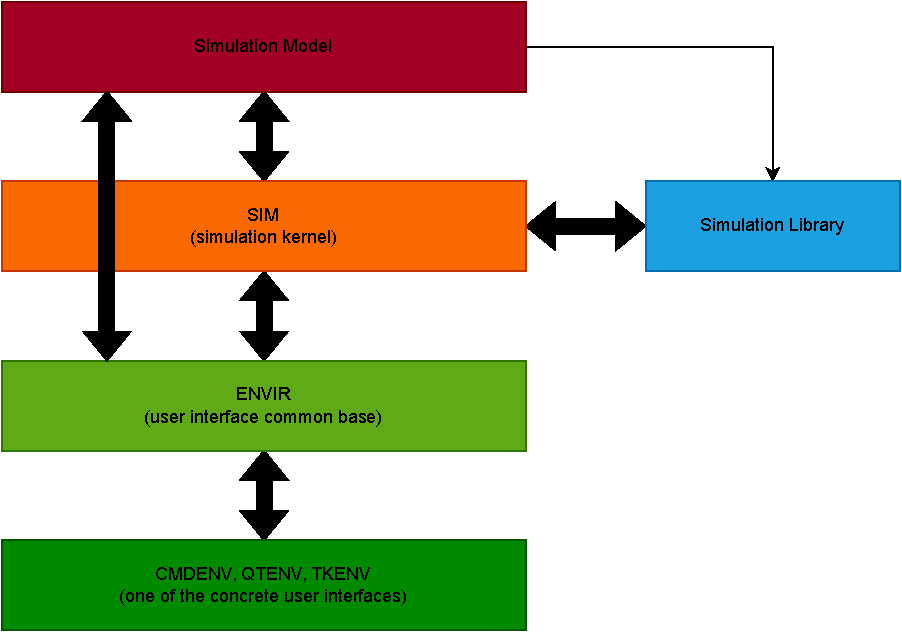
\includegraphics[width=0.5\textwidth]{opparch}
	\caption{OMNeT++ architecture. The Simulation Model extends classes
	provided by the Simulation Library to implement functionality. The
	Simulation Kernel is responsible for the execution of the simulation
	and event scheduling. Different user interfaces can be used to monitor
	the execution.}\label{fig:omnetpp-architecture}
\end{figure}

\ldots TODO \ldots

More information about \omnetpp{} can be found in the official website
\cite{omnetpp-website}, in the simulation manual
\cite{omnetpp-simulation-manual}, and in the paper by \citeauthor{omnetpp}
\cite{omnetpp}.
